\documentclass{article}

% content/resources/templates/preamble.tex
\usepackage[margin=0.6in]{geometry}
\author{Milav Dabgar}
\usepackage{amsmath,amssymb,amsthm}
\usepackage{booktabs}
\usepackage{multirow}
\usepackage{xcolor}
\usepackage{tcolorbox}
\tcbuselibrary{breakable,skins}
\usepackage[colorlinks=true,linkcolor=blue]{hyperref}
\usepackage{titlesec}
\usepackage{enumitem}
\usepackage{tikz}
\usepackage{pgfplots}
\usepackage{circuitikz}
\usepackage[version=4]{mhchem}
\usepackage{longtable}
\usepackage{array}
\usepackage{float}
\usepackage{caption}
\usepackage{listings}

\lstset{
  basicstyle=\small\ttfamily,
  breaklines=true,
  breakatwhitespace=false,
  postbreak=\mbox{\textcolor{red}{$\hookrightarrow$}\space},
  float=false,
  numbers=left,
  numberstyle=\tiny\color{gray},
  numbersep=10pt,
  xleftmargin=2em,
  keywordstyle=\color{blue},
  commentstyle=\color{green!60!black},
  stringstyle=\color{purple},
  backgroundcolor=\color{gray!5},
  showstringspaces=false,
  tabsize=2,
  captionpos=b,
  keepspaces=true,
  columns=flexible
}

\pgfplotsset{compat=1.18}
\usetikzlibrary{shapes,arrows,positioning,calc,patterns,decorations.pathmorphing,decorations.markings,arrows.meta}

% Color scheme
\definecolor{headcolor}{RGB}{0,102,204}
\definecolor{keycolor}{RGB}{220,20,60}
\definecolor{solutioncolor}{RGB}{34,139,34}
\definecolor{mnemoniccolor}{RGB}{148,0,211}
\definecolor{codecolor}{RGB}{0,0,100}

% Spacing
\setlength{\parskip}{3pt}
\setlist[itemize]{nosep}
\setlist[enumerate]{nosep}

% Title formatting
\titleformat{\section}{\Large\bfseries\color{headcolor}}{\thesection}{1em}{}
\titleformat{\subsection}{\large\bfseries\color{headcolor}}{\thesubsection}{1em}{}

% Pandoc tightlist compatibility
\providecommand{\tightlist}{%
  \setlength{\itemsep}{0pt}\setlength{\parskip}{0pt}}

% Pandoc longtable compatibility
\newcounter{none}
\def\thenone{}


% content/resources/templates/english-boxes.tex

% Custom environments
\newtcolorbox{solutionbox}{
 breakable,
 enhanced,
 colback=solutioncolor!5!white,
 colframe=solutioncolor!75!black,
 fonttitle=\bfseries,
 title=Solution
}

\newtcolorbox{solutionboxnobreak}{
 colback=solutioncolor!5!white,
 colframe=solutioncolor!75!black,
 fonttitle=\bfseries,
 title=Solution
}

\newtcolorbox{keyformula}{
 breakable,
 enhanced,
 colback=keycolor!5!white,
 colframe=keycolor!75!black,
 fonttitle=\bfseries,
 title=Key Formula
}

\newtcolorbox{mnemonicboxenv}{
 breakable,
 enhanced,
 colback=mnemoniccolor!5!white,
 colframe=mnemoniccolor!75!black,
 fonttitle=\bfseries,
 title=Mnemonic
}

\newcommand{\mnemonicbox}[1]{%
  \begin{mnemonicboxenv}
    #1
  \end{mnemonicboxenv}
}


% Custom commands for GTU solutions
% This file defines semantic commands for consistent formatting

% Question command with automatic formatting
\newcommand{\question}[2]{%
  \section*{Question #1}%
  \textbf{#2}%
}

% OR question variant
\newcommand{\questionor}[2]{%
  \section*{Question #1 OR}%
  \textbf{#2}%
}

% Proper table environment with caption
\newenvironment{answertable}[1]{%
  \begin{table}[htbp]
  \centering
  \caption{#1}
}{%
  \end{table}
}

% Proper figure environment for diagrams
\newenvironment{answerdiagram}[1]{%
  \begin{figure}[htbp]
  \centering
  \caption{#1}
}{%
  \end{figure}
}

% Semantic markup for key terms
\newcommand{\keyword}[1]{\textbf{#1}}
\newcommand{\code}[1]{\texttt{#1}}
\newcommand{\classname}[1]{\texttt{#1}}
\newcommand{\methodname}[1]{\texttt{#1}}

% Proper quotation marks
\newcommand{\mnemonic}[1]{``#1''}


\title{Microprocessor \& Microcontroller Systems (1333202) - Summer 2025 Solution}
\date{May 13, 2025}

\begin{document}
\maketitle

\questionmarks{1(A)}{3}{Draw The Bus Organization Of 8085.}

\begin{solutionbox}
\begin{center}
\begin{tikzpicture}[node distance=2cm]
    \node [gtu block, minimum width=3cm, minimum height=2cm] (mp) {8085 CPU};
    
    % Address Bus
    \draw [gtu arrow, ->] ($(mp.east) + (0, 0.5)$) -- ++(2,0) node[right] {Address Bus (16-bit) [Unidirectional]};
    
    % Data Bus
    \draw [gtu arrow, <->] (mp.east) -- ++(2,0) node[right] {Data Bus (8-bit) [Bidirectional]};
    
    % Control Bus
    \draw [gtu arrow, ->] ($(mp.east) + (0, -0.5)$) -- ++(2,0) node[right] {Control Bus (Rules) [Output/Input]};
    
    \node [right=0.5cm of mp.north east] {To Memory \& I/O};
\end{tikzpicture}
\captionof{figure}{8085 Bus Organization}
\end{center}

\textbf{Bus Types:}
\begin{itemize}
    \item \textbf{Address Bus}: 16-bit unidirectional bus for memory addressing.
    \item \textbf{Data Bus}: 8-bit bidirectional bus for data transfer.
    \item \textbf{Control Bus}: Control signals like RD, WR, ALE, IO/M.
\end{itemize}

\begin{mnemonicbox}ADC - Address, Data, Control\end{mnemonicbox}
\end{solutionbox}

\questionmarks{1(B)}{4}{Compare Microprocessor With Microcontroller.}

\begin{solutionbox}
\begin{center}
\captionof{table}{Microprocessor vs Microcontroller}
\begin{tabulary}{\linewidth}{|L|L|L|}
\hline
\textbf{Feature} & \textbf{Microprocessor} & \textbf{Microcontroller} \\ \hline
\textbf{Architecture} & External components needed. & All components on single chip. \\ \hline
\textbf{Memory} & External RAM/ROM required. & Internal RAM/ROM available. \\ \hline
\textbf{Cost} & Higher system cost. & Lower system cost. \\ \hline
\textbf{Power} & Higher power consumption. & Lower power consumption. \\ \hline
\textbf{Size} & Larger system size. & Compact system. \\ \hline
\textbf{Applications} & General purpose computing. & Embedded control applications. \\ \hline
\end{tabulary}
\end{center}

\textbf{Key Points:}
\begin{itemize}
    \item \textbf{Microprocessor}: CPU only, requires external support chips.
    \item \textbf{Microcontroller}: Complete computer system on chip.
\end{itemize}

\begin{mnemonicbox}MICRO - Memory Internal, Compact, Reduced cost, Optimized\end{mnemonicbox}
\end{solutionbox}

\questionmarks{1(C)}{7}{Draw And Explain Each Block Of 8085 Microprocessor.}

\begin{solutionbox}
\begin{center}
\begin{tikzpicture}[scale=0.8, transform shape]
    % Main Blocks
    \node [gtu block] (alu) {ALU (8-bit)};
    \node [gtu block, below=1cm of alu] (acc) {Accumulator (A)};
    \node [gtu block, below=0.5cm of acc] (temp) {Temp Reg};
    \node [gtu block, right=1cm of acc] (flags) {Flag Register};
    
    \node [gtu block, right=3cm of alu, minimum width=3cm] (regs) {Register Array\\B, C, D, E, H, L\\SP, PC};
    
    \node [gtu block, left=2cm of acc] (id) {Instruction\\Decoder};
    \node [gtu block, below=1cm of id] (timing) {Timing \&\\Control Unit};
    
    \node [gtu block, above=1cm of regs] (interrupt) {Interrupt Control};
    \node [gtu block, above=1cm of alu] (serial) {Serial I/O Control};
    
    % Connections
    \draw [gtu arrow, <->] (alu) -- (acc);
    \draw [gtu arrow] (alu) -- (flags);
    \draw [gtu arrow] (id) -- (timing);
    \draw [gtu arrow, <->] (alu) -- (regs);
    
    % Buses
    \draw [->, thick] (regs.east) -- ++(1,0) node[right] {Address/Data Bus};
    \draw [->, thick] (timing.south) -- ++(0,-1) node[below] {Control Signals};
    
\end{tikzpicture}
\captionof{figure}{8085 Block Diagram}
\end{center}

\textbf{Block Functions:}
\begin{itemize}
    \item \textbf{ALU}: Performs arithmetic and logical operations.
    \item \textbf{Accumulator}: Primary working register for data processing.
    \item \textbf{Register Array}: B, C, D, E, H, L general purpose registers.
    \item \textbf{Program Counter}: Holds address of next instruction.
    \item \textbf{Stack Pointer}: Points to top of stack in memory.
    \item \textbf{Control Unit}: Controls overall operation of processor.
\end{itemize}

\begin{mnemonicbox}APRIL - ALU, Program counter, Registers, Instruction decoder, Logic control\end{mnemonicbox}
\end{solutionbox}

\questionmarks{1(C) OR}{7}{Draw Pin Diagram Of 8085 Microprocessor And Explain Any 4(Four) Pins.}

\begin{solutionbox}
\begin{center}
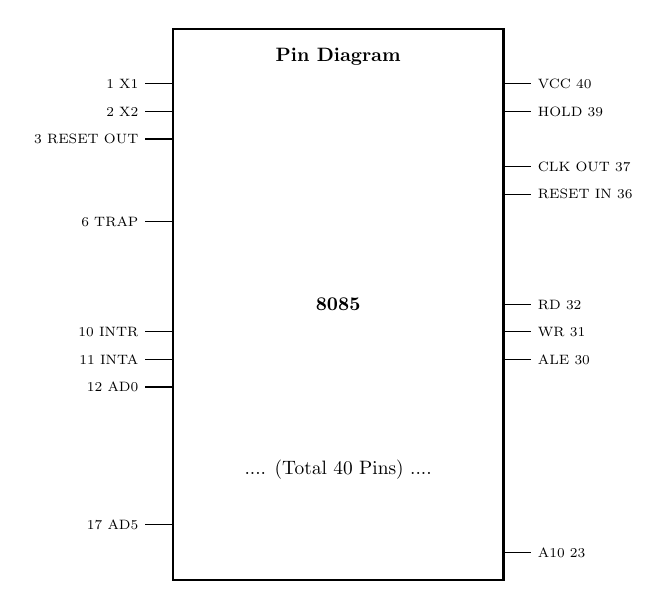
\begin{tikzpicture}[scale=0.7, transform shape]
    \draw [thick] (0,0) rectangle (6,10);
    \node at (3,5) {\textbf{8085}};
    \node at (3,9.5) {\textbf{Pin Diagram}};
    
    % Left Pins (Sample)
    \foreach \y/\label/\pin in {9/X1/1, 8.5/X2/2, 8/RESET OUT/3, 6.5/TRAP/6, 4.5/INTR/10, 4/INTA/11, 3.5/AD0/12, 1/AD5/17}
        \draw (-0.5, \y) node[left] {\scriptsize \pin\ \label} -- (0, \y);
        
    % Right Pins (Sample)
    \foreach \y/\label/\pin in {9/VCC/40, 8.5/HOLD/39, 7.5/CLK OUT/37, 7/RESET IN/36, 5/RD/32, 4.5/WR/31, 4/ALE/30, 0.5/A10/23}
        \draw (6, \y) -- (6.5, \y) node[right] {\scriptsize \label\ \pin};
        
    \node at (3,2) {.... (Total 40 Pins) ....};
\end{tikzpicture}
\captionof{figure}{8085 Pin Diagram}
\end{center}

\textbf{Pin Explanations:}
\begin{itemize}
    \item \textbf{ALE (Pin 30)}: Address Latch Enable - separates address and data on multiplexed bus.
    \item \textbf{RD (Pin 32)}: Read control signal - active low, indicates read operation.
    \item \textbf{WR (Pin 31)}: Write control signal - active low, indicates write operation.
    \item \textbf{RESET (Pin 36)}: Reset input - initializes processor when low.
\end{itemize}

\begin{mnemonicbox}ARWA - ALE, Read, Write, rAset\end{mnemonicbox}
\end{solutionbox}

\questionmarks{2(A)}{3}{Define : (1) Opcode (2) Operand}

\begin{solutionbox}
\textbf{Definitions:}
\begin{itemize}
    \item \textbf{Opcode}: Operation Code - specifies the operation to be performed (ADD, MOV, JMP).
    \item \textbf{Operand}: Data or address on which operation is performed.
\end{itemize}

\textbf{Example:}
\begin{verbatim}
MOV A, B
 |   |  |
 |   |  +-- Operand 2 (Source)  
 |   +-- Operand 1 (Destination)
 +-- Opcode
\end{verbatim}

\begin{mnemonicbox}OO - Operation + Operand\end{mnemonicbox}
\end{solutionbox}

\questionmarks{2(B)}{4}{Give Differences Between RISC And CISC.}

\begin{solutionbox}
\begin{center}
\captionof{table}{RISC vs CISC}
\begin{tabulary}{\linewidth}{|L|L|L|}
\hline
\textbf{Feature} & \textbf{RISC} & \textbf{CISC} \\ \hline
\textbf{Instructions} & Simple, fixed format. & Complex, variable format. \\ \hline
\textbf{Execution} & Single cycle execution. & Multiple cycle execution. \\ \hline
\textbf{Addressing} & Few addressing modes. & Many addressing modes. \\ \hline
\textbf{Memory} & Load/Store architecture. & Memory-to-memory operations. \\ \hline
\textbf{Compiler} & Complex compiler design. & Simple compiler design. \\ \hline
\end{tabulary}
\end{center}

\textbf{Key Points:}
\begin{itemize}
    \item \textbf{RISC}: Reduced Instruction Set Computer - simpler, faster.
    \item \textbf{CISC}: Complex Instruction Set Computer - feature rich.
\end{itemize}

\begin{mnemonicbox}RISC is SLIM - Simple, Load-store, Instruction reduced, Memory efficient\end{mnemonicbox}
\end{solutionbox}

\questionmarks{2(C)}{7}{Give Differences Between Von-Neumann \& Harvard Architecture.}

\begin{solutionbox}
\begin{center}
\begin{tikzpicture}[node distance=2cm]
    \node [gtu block] (cpu1) {CPU};
    \node [gtu block, right=of cpu1] (mem1) {Data + Instr\\Memory};
    \draw [gtu arrow, <->] (cpu1) -- node[above] {Single Bus} (mem1);
    \node [below=0.5cm of cpu1] {Von-Neumann};
    
    \node [gtu block, right=4cm of cpu1] (cpu2) {CPU};
    \node [gtu block, above right=0.5cm and 1.5cm of cpu2] (imem) {Instr Mem};
    \node [gtu block, below right=0.5cm and 1.5cm of cpu2] (dmem) {Data Mem};
    
    \draw [gtu arrow, <->] (cpu2) |- (imem);
    \draw [gtu arrow, <->] (cpu2) |- (dmem);
    
    \node [below=2cm of cpu2] {Harvard};
\end{tikzpicture}
\captionof{figure}{Von-Neumann vs Harvard}
\end{center}

\begin{center}
\captionof{table}{Architecture Comparison}
\begin{tabulary}{\linewidth}{|L|L|L|}
\hline
\textbf{Feature} & \textbf{Von-Neumann} & \textbf{Harvard} \\ \hline
\textbf{Memory} & Single memory for data and instructions. & Separate memory for data and instructions. \\ \hline
\textbf{Bus Structure} & Single bus system. & Dual bus system. \\ \hline
\textbf{Access} & Sequential access to data and instructions. & Simultaneous access possible. \\ \hline
\textbf{Cost} & Lower cost. & Higher cost. \\ \hline
\textbf{Speed} & Slower due to bus conflicts. & Faster parallel access. \\ \hline
\textbf{Examples} & 8085, General computers. & 8051, DSP processors. \\ \hline
\end{tabulary}
\end{center}

\begin{mnemonicbox}VH - Von has one bus, Harvard has two\end{mnemonicbox}
\end{solutionbox}

\questionmarks{2(A) OR}{3}{Define : (1) T-State (2) Instruction Cycle (3) Machine Cycle}

\begin{solutionbox}
\textbf{Definitions:}
\begin{itemize}
    \item \textbf{T-State}: Time state - basic timing unit, one clock period.
    \item \textbf{Instruction Cycle}: Complete execution of one instruction.
    \item \textbf{Machine Cycle}: Group of T-states required for one memory operation.
\end{itemize}

\textbf{Relationship:}
\begin{itemize}
    \item Instruction Cycle = Multiple Machine Cycles
    \item Machine Cycle = Multiple T-States (3-6 T-states)
\end{itemize}

\begin{mnemonicbox}TIM - T-state, Instruction cycle, Machine cycle\end{mnemonicbox}
\end{solutionbox}

\questionmarks{2(B) OR}{4}{Explain De-Multiplexing Of Address And Data Bus Of 8085.}

\begin{solutionbox}
\begin{center}
\begin{tikzpicture}[node distance=2.5cm]
    \node [gtu block, minimum height=3cm] (cpu) {8085\\CPU};
    \node [gtu block, right=3cm of cpu] (latch) {74LS373\\Latch};
    
    % Lines
    \draw [->, thick] ($(cpu.east)+(0,0.5)$) -- node[above] {AD0-AD7} ($(latch.west)+(0,0.5)$);
    \draw [->, thick] ($(cpu.east)+(0,-0.5)$) -- node[below] {ALE} ($(latch.west)+(0,-0.5)$);
    
    % Outputs
    \draw [->, thick] (latch.east) -- ++(1,0) node[right] {A0-A7 (Address)};
    \draw [->, thick] ($(latch.west)+(0.5,0.5)$) -- ++(0,-1.5) -- ++(2.5,0) node[right] {D0-D7 (Data)};
    
\end{tikzpicture}
\captionof{figure}{Demultiplexing Circuit}
\end{center}

\textbf{Process:}
\begin{itemize}
    \item \textbf{Step 1}: During T1, AD0-AD7 contains lower 8-bit address.
    \item \textbf{Step 2}: ALE goes high, latches address in external latch.
    \item \textbf{Step 3}: AD0-AD7 becomes data bus for remaining T-states.
\end{itemize}

\textbf{Components Required:}
\begin{itemize}
    \item \textbf{74LS373}: Octal latch IC for address latching.
    \item \textbf{ALE}: Address Latch Enable signal for timing.
\end{itemize}

\begin{mnemonicbox}LAD - Latch Address with Data separation\end{mnemonicbox}
\end{solutionbox}




\questionmarks{2(C) OR}{7}{Draw And Explain Flag Register Of 8085.}

\begin{solutionbox}
\begin{center}
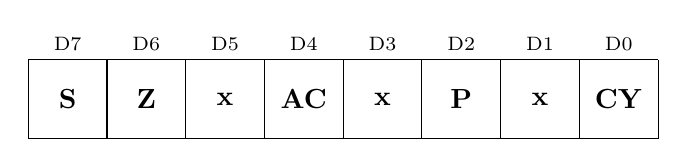
\begin{tikzpicture}
    % Flag Register
    \draw (0,0) grid (8,1);
    \foreach \x/\label in {0.5/D7, 1.5/D6, 2.5/D5, 3.5/D4, 4.5/D3, 5.5/D2, 6.5/D1, 7.5/D0}
        \node [above] at (\x, 1) {\scriptsize \label};
        
    \foreach \x/\val in {0.5/S, 1.5/Z, 2.5/x, 3.5/AC, 4.5/x, 5.5/P, 6.5/x, 7.5/CY}
        \node at (\x, 0.5) {\textbf{\val}};
\end{tikzpicture}
\captionof{figure}{Flag Register Format}
\end{center}

\textbf{Flag Descriptions:}
\begin{itemize}
    \item \textbf{CY (D0)}: Carry flag - Set when carry occurs.
    \item \textbf{P (D2)}: Parity flag - Set for even parity.
    \item \textbf{AC (D4)}: Auxiliary carry - Set for BCD operations.
    \item \textbf{Z (D6)}: Zero flag - Set when result is zero.
    \item \textbf{S (D7)}: Sign flag - Set when result is negative.
\end{itemize}

\textbf{Flag Operations:}
\begin{itemize}
    \item \textbf{Conditional Jumps}: Based on flag status (JZ, JC, JP).
    \item \textbf{Arithmetic Results}: Automatically updated after ALU operations.
\end{itemize}

\begin{mnemonicbox}SZAPC - Sign, Zero, Auxiliary, Parity, Carry\end{mnemonicbox}
\end{solutionbox}



\questionmarks{3(A)}{3}{What Is SFR ? List Out Any Three SFR.}

\begin{solutionbox}
\textbf{SFR Definition:}
\textbf{Special Function Register} - Dedicated registers with specific functions in microcontroller.

\textbf{Three SFRs:}
\begin{itemize}
    \item \textbf{ACC (E0H)}: Accumulator register.
    \item \textbf{PSW (D0H)}: Program Status Word.
    \item \textbf{SP (81H)}: Stack Pointer register.
\end{itemize}

\textbf{Characteristics:}
\begin{itemize}
    \item \textbf{Address Range}: 80H to FFH in internal RAM.
    \item \textbf{Bit Addressable}: Some SFRs allow individual bit access.
    \item \textbf{Function Specific}: Each has dedicated hardware function.
\end{itemize}

\begin{mnemonicbox}APS - ACC, PSW, Stack Pointer\end{mnemonicbox}
\end{solutionbox}

\questionmarks{3(B)}{4}{Explain Program Counter (PC) And Data Pointer (DPTR) Register.}

\begin{solutionbox}
\textbf{Program Counter (PC):}
\begin{itemize}
    \item \textbf{Size}: 16-bit register.
    \item \textbf{Function}: Holds address of next instruction to be executed.
    \item \textbf{Auto-increment}: Automatically increments after instruction fetch.
    \item \textbf{Range}: 0000H to FFFFH.
\end{itemize}

\textbf{Data Pointer (DPTR):}
\begin{itemize}
    \item \textbf{Size}: 16-bit register (DPH + DPL).
    \item \textbf{Function}: Points to external data memory locations.
    \item \textbf{Usage}: Used with MOVX instructions for external memory access.
    \item \textbf{Components}: DPH (83H) and DPL (82H).
\end{itemize}

\begin{center}
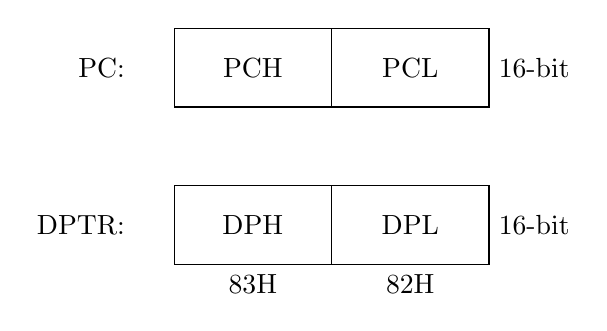
\begin{tikzpicture}
    % PC
    \node [anchor=east] at (0,1) {PC:};
    \draw (0.5,0.5) rectangle (2.5,1.5) node[midway] {PCH};
    \draw (2.5,0.5) rectangle (4.5,1.5) node[midway] {PCL};
    \node [right] at (4.5,1) {16-bit};
    
    % DPTR
    \node [anchor=east] at (0,-1) {DPTR:};
    \draw (0.5,-1.5) rectangle (2.5,-0.5) node[midway] {DPH};
    \draw (2.5,-1.5) rectangle (4.5,-0.5) node[midway] {DPL};
    \node [right] at (4.5,-1) {16-bit};
    \node [below] at (1.5,-1.5) {83H};
    \node [below] at (3.5,-1.5) {82H};
\end{tikzpicture}
\captionof{figure}{PC and DPTR Registers}
\end{center}

\begin{mnemonicbox}PD - PC Points to Program, DPTR Points to Data\end{mnemonicbox}
\end{solutionbox}

\questionmarks{3(C)}{7}{Draw And Explain Architecture Of 8051.}

\begin{solutionbox}
\begin{center}
\begin{tikzpicture}[scale=0.8, transform shape]
    % CPU Core
    \node [gtu block] (alu) {ALU (8-bit)};
    \node [gtu block, below=1cm of alu] (acc) {A};
    \node [gtu block, left=0.5cm of acc] (b) {B};
    \node [gtu block, right=0.5cm of acc] (psw) {PSW};
    
    % Memory / SFRs
    \node [gtu block, right=3cm of alu] (ram) {128B RAM};
    \node [gtu block, below=0.5cm of ram] (rom) {4KB ROM};
    \node [gtu block, above=0.5cm of ram] (sfr) {SFR Area};
    
    % Peripherals
    \node [gtu block, left=3cm of alu] (timer) {Timer 0, 1};
    \node [gtu block, below=0.5cm of timer] (serial) {Serial Port};
    \node [gtu block, above=0.5cm of timer] (int) {Interrupts};
    
    % IO Ports
    \node [gtu block, below=3cm of acc, minimum width=6cm] (ports) {I/O Ports P0, P1, P2, P3};
    
    % Connections (Simplified)
    \draw [gtu arrow, <->] (alu) -- (acc);
    \draw [gtu arrow] (alu) -- (b);
    \draw [gtu arrow] (alu) -- (psw);
    
    \draw [gtu arrow, <->] (acc) -- (ram);
    \draw [gtu arrow, <->] (ram) -- (sfr);
    
    \draw [gtu arrow, <->] (sfr) -| (timer);
    \draw [gtu arrow, <->] (sfr) -| (serial);
    \draw [gtu arrow, <->] (int) -- (alu);
    
    \draw [gtu arrow, <->] (alu) -- (ports);
\end{tikzpicture}
\captionof{figure}{8051 Architecture Block Diagram}
\end{center}

\textbf{Architecture Components:}
\begin{itemize}
    \item \textbf{CPU}: 8-bit ALU with accumulator and B register.
    \item \textbf{Memory}: 4KB internal ROM, 128B internal RAM.
    \item \textbf{I/O Ports}: Four 8-bit bidirectional ports (P0-P3).
    \item \textbf{Timers}: Two 16-bit timers/counters (T0, T1).
    \item \textbf{Serial Port}: Full duplex UART for communication.
    \item \textbf{Interrupts}: 5 interrupt sources with priority levels.
\end{itemize}

\textbf{Special Features:}
\begin{itemize}
    \item \textbf{Boolean Processor}: Bit manipulation capabilities.
    \item \textbf{Addressing Modes}: 8 different addressing modes.
    \item \textbf{Power Management}: Idle and power-down modes.
\end{itemize}

\begin{mnemonicbox}MIPTIS - Memory, I/O, Processor, Timers, Interrupts, Serial\end{mnemonicbox}
\end{solutionbox}

\questionmarks{3(A) OR}{3}{Explain Following Pins Of 8051: (1) ALE (2) PSEN (3) XTAL1 \& XTAL2}

\begin{solutionbox}
\textbf{Pin Functions:}
\begin{itemize}
    \item \textbf{ALE (Pin 30)}: Address Latch Enable
    \begin{itemize}
        \item Output pulse for latching lower address byte.
        \item Active high signal at 1/6 of oscillator frequency.
    \end{itemize}
    
    \item \textbf{PSEN (Pin 29)}: Program Store Enable
    \begin{itemize}
        \item Active low output for external program memory read.
        \item Connected to OE pin of external EPROM.
    \end{itemize}
    
    \item \textbf{XTAL1 \& XTAL2 (Pins 19, 18)}: Crystal connections
    \begin{itemize}
        \item Connect external crystal for clock generation.
        \item Typical frequency: 11.0592 MHz or 12 MHz.
    \end{itemize}
\end{itemize}

\begin{center}
\begin{circuitikz}
    \draw (0,0) node[draw, minimum width=3cm, minimum height=1cm] (ic) {8051};
    \draw (ic.south west) ++(0.5,0) -- ++(0,-0.5) node[below] {XTAL1}; 
    \draw (ic.south east) ++(-0.5,0) -- ++(0,-0.5) node[below] {XTAL2};
    
    \coordinate (x1) at ($(ic.south west) + (0.5,-1)$);
    \coordinate (x2) at ($(ic.south east) + (-0.5,-1)$);
    
    \draw (x1) -- node[midway, fill=white, draw] {Crystal} (x2);
    \draw (x1) to[C, l=33pF] ++(0,-1.5) node[ground]{};
    \draw (x2) to[C, l=33pF] ++(0,-1.5) node[ground]{};
    
    \draw ($(ic.south west) + (0.5,-0.5)$) -- (x1);
    \draw ($(ic.south east) + (-0.5,-0.5)$) -- (x2);
\end{circuitikz}
\captionof{figure}{Crystal Oscillator Connection}
\end{center}

\begin{mnemonicbox}APX - ALE latches Address, PSEN enables Program, XTAL generates clocK\end{mnemonicbox}
\end{solutionbox}

\questionmarks{3(B) OR}{4}{Describe Internal RAM Organization Of 8051 Microcontroller.}

\begin{solutionbox}
\begin{center}
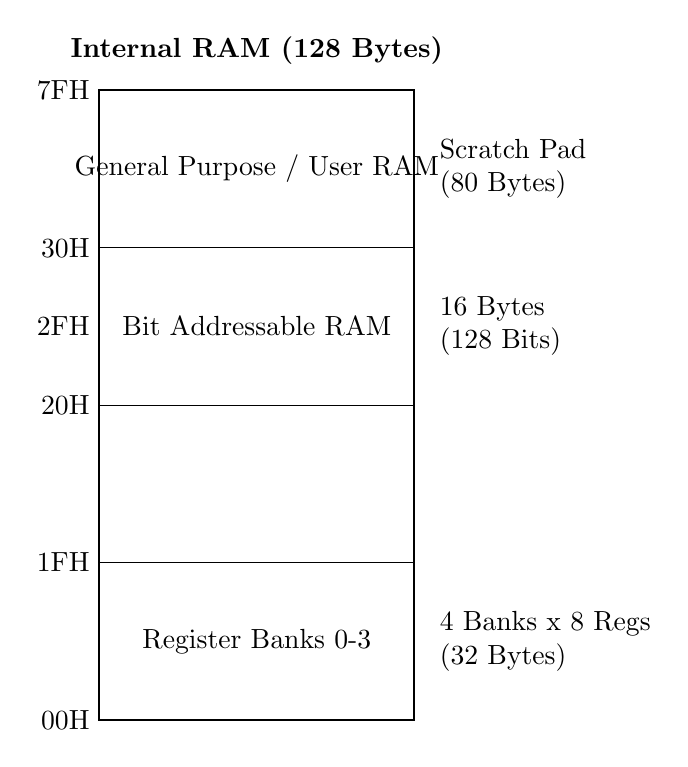
\begin{tikzpicture}
    % RAM Memory Map
    \draw [thick] (0,0) rectangle (4,8);
    \node at (2,8.5) {\textbf{Internal RAM (128 Bytes)}};
    
    % Sections
    \draw (0,6) -- (4,6);
    \draw (0,4) -- (4,4);
    \draw (0,2) -- (4,2);
    \draw (0,0) -- (4,0);
    
    % Labels
    \node at (2,7) {General Purpose / User RAM};
    \node at (2,5) {Bit Addressable RAM};
    \node at (2,1) {Register Banks 0-3};
    
    % Addresses
    \node [anchor=east] at (0,8) {7FH};
    \node [anchor=east] at (0,6) {30H};
    \node [anchor=east] at (0,5) {2FH};
    \node [anchor=east] at (0,4) {20H};
    \node [anchor=east] at (0,2) {1FH};
    \node [anchor=east] at (0,0) {00H};
    
    % Details
    \node [right, align=left] at (4.2, 7) {Scratch Pad\\(80 Bytes)};
    \node [right, align=left] at (4.2, 5) {16 Bytes\\(128 Bits)};
    \node [right, align=left] at (4.2, 1) {4 Banks x 8 Regs\\(32 Bytes)};
\end{tikzpicture}
\captionof{figure}{8051 Internal RAM Organization}
\end{center}

\textbf{RAM Sections:}
\begin{itemize}
    \item \textbf{Register Banks}: 4 banks $\times$ 8 registers each (00H-1FH).
    \item \textbf{Bit Addressable}: 16 bytes with individual bit access (20H-2FH).
    \item \textbf{General Purpose}: 80 bytes for user data (30H-7FH).
    \item \textbf{Stack Area}: Usually starts from 08H upward.
\end{itemize}

\textbf{Addressing:}
\begin{itemize}
    \item \textbf{Direct}: Using actual address (MOV 30H, A).
    \item \textbf{Indirect}: Using register pointer (MOV @R0, A).
\end{itemize}

\begin{mnemonicbox}RBGS - Register banks, Bit addressable, General purpose, Stack\end{mnemonicbox}
\end{solutionbox}

\questionmarks{3(C) OR}{7}{Draw Pin Diagram Of 8051 And Explain Any 04(Four) Pins.}

\begin{solutionbox}
\begin{center}
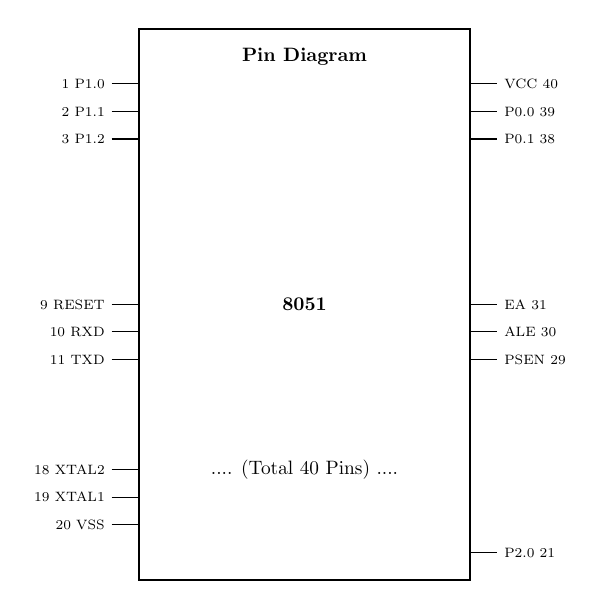
\begin{tikzpicture}[scale=0.7, transform shape]
    \draw [thick] (0,0) rectangle (6,10);
    \node at (3,5) {\textbf{8051}};
    \node at (3,9.5) {\textbf{Pin Diagram}};
    
    % Left Pins
    \foreach \y/\label/\pin in {9/P1.0/1, 8.5/P1.1/2, 8/P1.2/3, 5/RESET/9, 4.5/RXD/10, 4/TXD/11, 2/XTAL2/18, 1.5/XTAL1/19, 1/VSS/20}
        \draw (-0.5, \y) node[left] {\scriptsize \pin\ \label} -- (0, \y);
        
    % Right Pins
    \foreach \y/\label/\pin in {9/VCC/40, 8.5/P0.0/39, 8/P0.1/38, 5/EA/31, 4.5/ALE/30, 4/PSEN/29, 0.5/P2.0/21}
        \draw (6, \y) -- (6.5, \y) node[right] {\scriptsize \label\ \pin};
        
    \node at (3,2) {.... (Total 40 Pins) ....};
\end{tikzpicture}
\captionof{figure}{8051 Pin Diagram}
\end{center}

\textbf{Pin Explanations:}
\begin{itemize}
    \item \textbf{RESET (Pin 9)}: Reset input - Active high, initializes microcontroller.
    \item \textbf{EA/VPP (Pin 31)}: External Access - Controls program memory selection.
    \item \textbf{P0 (Pins 32-39)}: Port 0 - Multiplexed address/data bus for external memory.
    \item \textbf{P2 (Pins 21-28)}: Port 2 - High-order address bus for external memory.
\end{itemize}

\begin{mnemonicbox}REPP - REset, External Access, Port 0, Port 2\end{mnemonicbox}
\end{solutionbox}

\questionmarks{4(A)}{3}{Write A Program To Multiply Data Stored In R0 Register With Data Stored In R1 Register. Store The Result In R2 Register (LSB) And R3 Register (MSB).}

\begin{solutionbox}
\begin{lstlisting}[language={[x86masm]Assembler}, caption={Multiplication Program}]
    ORG 0000H
    MOV R0, #05H    ; Load first number
    MOV R1, #03H    ; Load second number
    MOV A, R0       ; Move R0 to accumulator
    MOV B, R1       ; Move R1 to B register
    MUL AB          ; Multiply A and B
    MOV R2, A       ; Store LSB in R2
    MOV R3, B       ; Store MSB in R3
    END
\end{lstlisting}

\textbf{Program Flow:}
\begin{itemize}
    \item \textbf{Load operands} into R0 and R1.
    \item \textbf{Transfer} to A and B registers for multiplication.
    \item \textbf{Execute} MUL AB instruction.
    \item \textbf{Store} 16-bit result (A=LSB, B=MSB).
\end{itemize}

\textbf{Result Storage:}
\begin{itemize}
    \item \textbf{R2}: Contains lower 8 bits of product.
    \item \textbf{R3}: Contains upper 8 bits of product.
\end{itemize}

\begin{mnemonicbox}LTSE - Load, Transfer, multiply, Store result\end{mnemonicbox}
\end{solutionbox}

\questionmarks{4(B)}{4}{List Out Data Transfer Instructions And Explain Any Two Data Transfer Instructions With Suitable Examples.}

\begin{solutionbox}
\textbf{Data Transfer Instructions:}
\begin{center}
\begin{tabulary}{\linewidth}{|L|L|}
\hline
\textbf{Instruction} & \textbf{Function} \\ \hline
MOV & Move data between registers/memory. \\ \hline
MOVX & Move data to/from external memory. \\ \hline
MOVC & Move code byte to accumulator. \\ \hline
PUSH & Push data onto stack. \\ \hline
POP & Pop data from stack. \\ \hline
XCH & Exchange accumulator with register. \\ \hline
XCHD & Exchange lower nibble. \\ \hline
\end{tabulary}
\end{center}

\textbf{Detailed Examples:}

\textbf{1. MOV Instruction:}
\begin{lstlisting}[language={[x86masm]Assembler}]
    MOV A, #50H     ; Load immediate data 50H into accumulator
    MOV R0, A       ; Copy accumulator content to R0
    MOV 30H, A      ; Store accumulator content at address 30H
\end{lstlisting}

\textbf{2. PUSH/POP Instructions:}
\begin{lstlisting}[language={[x86masm]Assembler}]
    PUSH ACC        ; Push accumulator onto stack
    PUSH 00H        ; Push R0 content onto stack
    POP 01H         ; Pop stack content to R1
    POP ACC         ; Pop stack content to accumulator
\end{lstlisting}

\begin{mnemonicbox}Move Makes Programs Possible - MOV, MOVX, PUSH, POP\end{mnemonicbox}
\end{solutionbox}

\questionmarks{4(C)}{7}{Define And Explain Addressing Modes Of 8051.}

\begin{solutionbox}
\textbf{8051 Addressing Modes:}
\begin{center}
\begin{tabulary}{\linewidth}{|L|L|L|L|}
\hline
\textbf{Mode} & \textbf{Description} & \textbf{Example} & \textbf{Usage} \\ \hline
\textbf{Immediate} & Data is part of instruction. & \code{MOV A, \#50H} & Constant values. \\ \hline
\textbf{Register} & Uses register directly. & \code{MOV A, R0} & Fast access. \\ \hline
\textbf{Direct} & Uses direct address. & \code{MOV A, 30H} & RAM locations. \\ \hline
\textbf{Indirect} & Uses register as pointer. & \code{MOV A, @R0} & Dynamic addressing. \\ \hline
\textbf{Indexed} & Base + offset addressing. & \code{MOVC A, @A+DPTR} & Table lookup. \\ \hline
\textbf{Relative} & PC + offset. & \code{SJMP LOOP} & Branch instructions. \\ \hline
\textbf{Absolute} & Direct jump address. & \code{LJMP 1000H} & Long jumps. \\ \hline
\textbf{Bit} & Individual bit access. & \code{SETB P1.0} & Control operations. \\ \hline
\end{tabulary}
\end{center}

\textbf{Detailed Examples:}
\begin{lstlisting}[language={[x86masm]Assembler}]
    ; Immediate Addressing
    MOV A, #25H         ; Load 25H into A
    
    ; Register Addressing
    MOV A, R1           ; Copy R1 to A
    
    ; Direct Addressing
    MOV A, 40H          ; Load from address 40H
    
    ; Indirect Addressing
    MOV R0, #40H        ; R0 points to 40H
    MOV A, @R0          ; Load from address pointed by R0
    
    ; Indexed Addressing
    MOV DPTR, #TABLE    ; Point to table
    MOV A, #02H         ; Index value
    MOVC A, @A+DPTR     ; Load from TABLE+2
\end{lstlisting}

\begin{mnemonicbox}IRIDRAB - Immediate, Register, Indirect, Direct, Relative, Absolute, Bit\end{mnemonicbox}
\end{solutionbox}

\questionmarks{4(A) OR}{3}{Write A Program To Find 2's Complement of Data Stored in R0 Register.}

\begin{solutionbox}
\begin{lstlisting}[language={[x86masm]Assembler}, caption={2's Complement Program}]
    ORG 0000H
    MOV R0, #85H        ; Load test data
    MOV A, R0           ; Copy data to accumulator
    CPL A               ; Complement all bits (1's complement)
    INC A               ; Add 1 to get 2's complement
    MOV R1, A           ; Store result in R1
    END
\end{lstlisting}

\textbf{Algorithm:}
\begin{itemize}
    \item \textbf{Step 1}: Load data from R0 to accumulator.
    \item \textbf{Step 2}: Complement all bits using CPL A.
    \item \textbf{Step 3}: Add 1 using INC A for 2's complement.
    \item \textbf{Step 4}: Store result back.
\end{itemize}

\textbf{Verification:}
\begin{verbatim}
Original: 85H = 10000101B
1's Comp: 7AH = 01111010B  
2's Comp: 7BH = 01111011B
\end{verbatim}

\begin{mnemonicbox}CCI - Complement, aCd 1, Include result\end{mnemonicbox}
\end{solutionbox}

\questionmarks{4(B) OR}{4}{List Logical Instructions And Explain Any Two Logical Instructions With Suitable Examples.}

\begin{solutionbox}
\textbf{Logical Instructions:}
\begin{center}
\begin{tabulary}{\linewidth}{|L|L|}
\hline
\textbf{Instruction} & \textbf{Function} \\ \hline
ANL & Logical AND operation. \\ \hline
ORL & Logical OR operation. \\ \hline
XRL & Logical XOR operation. \\ \hline
CPL & Complement operation. \\ \hline
RL/RLC & Rotate left. \\ \hline
RR/RRC & Rotate right. \\ \hline
SWAP & Swap nibbles. \\ \hline
\end{tabulary}
\end{center}

\textbf{Detailed Examples:}

\textbf{1. ANL (AND Logic):}
\begin{lstlisting}[language={[x86masm]Assembler}]
    MOV A, #0F0H        ; A = 11110000B
    ANL A, #0AAH        ; AND with 10101010B
                        ; Result: A = 10100000B = A0H
\end{lstlisting}
\textbf{Usage}: Masking specific bits, clearing unwanted bits.

\textbf{2. ORL (OR Logic):}
\begin{lstlisting}[language={[x86masm]Assembler}]
    MOV A, #0F0H        ; A = 11110000B  
    ORL A, #00FH        ; OR with 00001111B
                        ; Result: A = 11111111B = FFH
\end{lstlisting}
\textbf{Usage}: Setting specific bits, combining bit patterns.

\begin{mnemonicbox}AXOR - AND masks, XOR toggles, OR sets, Rotate shifts\end{mnemonicbox}
\end{solutionbox}

\questionmarks{4(C) OR}{7}{Explain Following Instructions: (1)ADDC (2) INC (3) DEC (4) JZ (5) SUBB (6) NOP (7) RET}

\begin{solutionbox}
\textbf{Instruction Explanations:}

\begin{enumerate}
    \item \textbf{ADDC (Add with Carry)}: Adds source, destination, and carry flag.
    \begin{lstlisting}[language={[x86masm]Assembler}]
    MOV A, #80H
    ADDC A, #90H    ; A = A + 90H + Carry flag
    \end{lstlisting}
    
    \item \textbf{INC (Increment)}: Increases operand by 1.
    \begin{lstlisting}[language={[x86masm]Assembler}]
    INC A           ; A = A + 1
    INC R0          ; R0 = R0 + 1
    \end{lstlisting}
    
    \item \textbf{DEC (Decrement)}: Decreases operand by 1.
    \begin{lstlisting}[language={[x86masm]Assembler}]
    DEC A           ; A = A - 1
    DEC R1          ; R1 = R1 - 1
    \end{lstlisting}
    
    \item \textbf{JZ (Jump on Zero)}: Conditional jump when zero flag is set.
    \begin{lstlisting}[language={[x86masm]Assembler}]
    DEC A
    JZ ZERO_LABEL   ; Jump if A = 0
    \end{lstlisting}
    
    \item \textbf{SUBB (Subtract with Borrow)}: Subtracts source and carry from accumulator.
    \begin{lstlisting}[language={[x86masm]Assembler}]
    MOV A, #50H
    SUBB A, #30H    ; A = A - 30H - Carry flag
    \end{lstlisting}
    
    \item \textbf{NOP (No Operation)}: Provides timing delay, placeholder.
    \begin{lstlisting}[language={[x86masm]Assembler}]
    NOP             ; Do nothing, consume 1 cycle
    \end{lstlisting}
    
    \item \textbf{RET (Return)}: Returns from subroutine to calling address.
    \begin{lstlisting}[language={[x86masm]Assembler}]
    CALL SUBROUTINE
    ...
    SUBROUTINE:
        RET         ; Return to caller
    \end{lstlisting}
\end{enumerate}

\begin{mnemonicbox}AIDS NR - Add, Increment, Decrement, Subtract, No-op, Return\end{mnemonicbox}
\end{solutionbox}

\questionmarks{5(A)}{3}{Explain DJNZ And CJNE Instructions With Suitable Examples.}

\begin{solutionbox}
\textbf{DJNZ (Decrement and Jump if Not Zero):}
\begin{lstlisting}[language={[x86masm]Assembler}]
    MOV R0, #05H        ; Initialize counter
    LOOP:
        MOV A, #00H     ; Some operation
        DJNZ R0, LOOP   ; Decrement R0, jump if not zero
\end{lstlisting}
\textbf{Function}: Combines decrement and conditional jump operations.

\textbf{CJNE (Compare and Jump if Not Equal):}
\begin{lstlisting}[language={[x86masm]Assembler}]
    MOV A, #30H
    CJNE A, #30H, NOT_EQUAL  ; Compare A with 30H
    MOV R0, #01H             ; Equal case
    SJMP CONTINUE
    NOT_EQUAL:
    MOV R0, #00H             ; Not equal case
    CONTINUE:
\end{lstlisting}
\textbf{Function}: Compares two operands and jumps if not equal.

\begin{mnemonicbox}DC - Decrement count, Compare jump\end{mnemonicbox}
\end{solutionbox}

\questionmarks{5(B)}{4}{Write An Assembly Language Program To Generate The Time Delay Of 30ms Using Timer 0. Assume Crystal Frequency Is 12 MHz}

\begin{solutionbox}
\begin{lstlisting}[language={[x86masm]Assembler}, caption={30ms Delay Program}]
    ORG 0000H
    MAIN:
        CALL DELAY_30MS     ; Call 30ms delay
        SJMP MAIN           ; Repeat
    
    DELAY_30MS:
        MOV TMOD, #01H      ; Timer 0, Mode 1 (16-bit)
        MOV TH0, #8AH       ; Load high byte for 30ms
        MOV TL0, #23H       ; Load low byte  
        SETB TR0            ; Start Timer 0
    WAIT:
        JNB TF0, WAIT       ; Wait for timer overflow
        CLR TR0             ; Stop timer
        CLR TF0             ; Clear timer flag
        RET
    END
\end{lstlisting}

\textbf{Calculation for 30ms delay:}
\begin{itemize}
    \item Crystal Frequency = 12 MHz
    \item Machine Cycle = 12/12 MHz = 1 $\mu$s
    \item For 30ms = 30,000 $\mu$s = 30,000 machine cycles
    \item Timer Count = $65536 - 30000 = 35536 = 8A23H$
    \item TH0 = 8AH, TL0 = 23H
\end{itemize}

\begin{mnemonicbox}CLSW - Calculate, Load, Start, Wait\end{mnemonicbox}
\end{solutionbox}

\questionmarks{5(C)}{7}{Draw The Interfacing Diagram Of LCD With 8051. Explain Pins Of LCD Which Are Necessary For Interfacing.}

\begin{solutionbox}
\begin{center}
\begin{circuitikz}
    \node [gtu block, minimum height=4cm] (lcd) {LCD 16x2};
    \node [gtu block, left=3cm of lcd, minimum height=4cm] (cpu) {8051};
    
    % Data Lines
    \draw [->, thick] (cpu.east) -- node[above] {D4-D7 (P2)} (lcd.west);
    
    % Control Lines
    \draw [->] ($(cpu.east)+(0,-1)$) -- node[below] {RS, RW, EN (P1)} ($(lcd.west)+(0,-1)$);
    
    % Power
    \draw ($(lcd.north)+(1,0)$) -- ++(0,0.5) node[vcc] {+5V};
    \draw ($(lcd.south)+(1,0)$) -- ++(0,-0.5) node[ground] {};
    
    % Potentiometer for Contrast
    \draw ($(lcd.south)+(-1,0)$) -- ++(0,-1) node[ground] {}; 
    \node [below right] at ($(lcd.south)+(-1,0)$) {VEE};
\end{circuitikz}
\captionof{figure}{LCD Interfacing}
\end{center}

\textbf{LCD Pin Functions:}
\begin{itemize}
    \item \textbf{RS (Pin 4)}: Register Select - 0=Command, 1=Data.
    \item \textbf{RW (Pin 5)}: Read/Write - 0=Write, 1=Read.
    \item \textbf{EN (Pin 6)}: Enable - High to low pulse for data transfer.
    \item \textbf{D4-D7 (Pins 11-14)}: 4-bit data lines for commands/data.
\end{itemize}

\textbf{Basic LCD Commands:}
\begin{itemize}
    \item \textbf{0x38}: Function set (8-bit, 2 lines).
    \item \textbf{0x0E}: Display ON, cursor ON.
    \item \textbf{0x01}: Clear display.
    \item \textbf{0x80}: Set cursor to first line.
\end{itemize}

\begin{mnemonicbox}REED - RS selects, RW reads, EN enables, Data transfers\end{mnemonicbox}
\end{solutionbox}

\questionmarks{5(A) OR}{3}{Write A Program To Perform OR Operation On Data Stored In 65h Memory Location With Data Stored In 75h Memory Location. Store The Result In R6 Register.}

\begin{solutionbox}
\begin{lstlisting}[language={[x86masm]Assembler}, caption={OR Operation Program}]
    ORG 0000H
    MOV 65H, #0F0H      ; Store test data at 65H
    MOV 75H, #0AAH      ; Store test data at 75H
    
    MOV A, 65H          ; Load data from 65H to accumulator
    ORL A, 75H          ; OR with data at 75H
    MOV R6, A           ; Store result in R6 register
    END
\end{lstlisting}

\textbf{Example Calculation:}
\begin{verbatim}
Data at 65H: F0H = 11110000B
Data at 75H: AAH = 10101010B  
OR Result:   FAH = 11111010B
\end{verbatim}

\begin{mnemonicbox}LOS - Load, OR, Store result\end{mnemonicbox}
\end{solutionbox}

\questionmarks{5(B) OR}{4}{Write An Assembly Language Program To Generate A Square Wave Of 2khz On P1.3. Crystal Frequency Is 11.0592 Mhz.}

\begin{solutionbox}
\begin{lstlisting}[language={[x86masm]Assembler}, caption={Square Wave Program}]
    ORG 0000H
    MAIN:
        SETB P1.3           ; Set P1.3 high
        CALL DELAY_250US    ; Delay for half period
        CLR P1.3            ; Set P1.3 low
        CALL DELAY_250US    ; Delay for half period
        SJMP MAIN           ; Repeat continuously
    
    DELAY_250US:
        MOV TMOD, #01H      ; Timer 0, Mode 1
        MOV TH0, #0FEH      ; Load high byte
        MOV TL0, #0CBH      ; Load low byte
        SETB TR0            ; Start Timer 0
    WAIT:
        JNB TF0, WAIT       ; Wait for overflow
        CLR TR0             ; Stop timer
        CLR TF0             ; Clear flag
        RET
    END
\end{lstlisting}

\textbf{Calculation for 2KHz Square Wave:}
\begin{itemize}
    \item Frequency = 2KHz, Period = 500$\mu$s. Half Period = 250$\mu$s.
    \item Crystal = 11.0592 MHz. Machine Cycle = 1.085$\mu$s.
    \item Timer Count = $250 / 1.085 \approx 230$.
    \item Timer Value = $65536 - 230 = 65306 = FECBH$.
\end{itemize}

\begin{mnemonicbox}SCDW - Set high, Clear low, Delay, Wait\end{mnemonicbox}
\end{solutionbox}

\questionmarks{5(C) OR}{7}{Draw \& Explain The Interfacing Of 7-Segment Display With 8051.}

\begin{solutionbox}
\begin{center}
\begin{circuitikz}
    \draw (0,0) node[draw, minimum height=2cm] (P1) {Port 1};
    \draw (4,0) node[draw, minimum height=2cm] (disp) {7-Seg};
    
    \foreach \y in {0.7, 0.5, 0.3, 0.1, -0.1, -0.3, -0.5, -0.7}
        \draw [->] ($(P1.east)+(0,\y)$) -- ($(disp.west)+(0,\y)$);
        
    \node [right=0.2cm of P1] {\scriptsize a-g, dp};
    \node [above] at (2, 0.8) {Current Limiting Resistors (330$\Omega$)};
\end{circuitikz}
\captionof{figure}{7-Segment Interface}
\end{center}

\textbf{Display Configuration:}
\begin{center}
\begin{tabulary}{\linewidth}{|L|L|L|}
\hline
\textbf{Digit} & \textbf{Common Cathode} & \textbf{Common Anode} \\ \hline
0 & 3FH & C0H \\ \hline
1 & 06H & F9H \\ \hline
2 & 5BH & A4H \\ \hline
\end{tabulary}
\end{center}

\textbf{Sample Program:}
\begin{lstlisting}[language={[x86masm]Assembler}]
    MOV DPTR, #DIGIT_TABLE  ; Point to lookup table
    MOV A, #05H             ; Display digit 5
    MOVC A, @A+DPTR         ; Get 7-segment code
    MOV P1, A               ; Send to display
\end{lstlisting}

\begin{mnemonicbox}CRAM - Common connection, Resistors limit, Address segments, Multiplex digits\end{mnemonicbox}
\end{solutionbox}

\end{document}

